\chapter{实验}
\label{chap:experiment}
在实验部分,我们通过让游戏AI对战固定场次来判断其强度。也就是说,若某个玩家的胜率越高,则其强度越强。由于缺乏职业玩家与普通玩家的大量数据,我们无法使用Elo rating对AI玩家的强度进行打分~\cite{glickman1999rating}。
在目前的硬件条件下,我们支持对角开局,如图~\ref{fig:sstate}~中所示。白色方总是先攻,对战双方每50局互换先手,每100局更换开局棋盘,一共对战400局。
\begin{figure}[H]
    \centering
    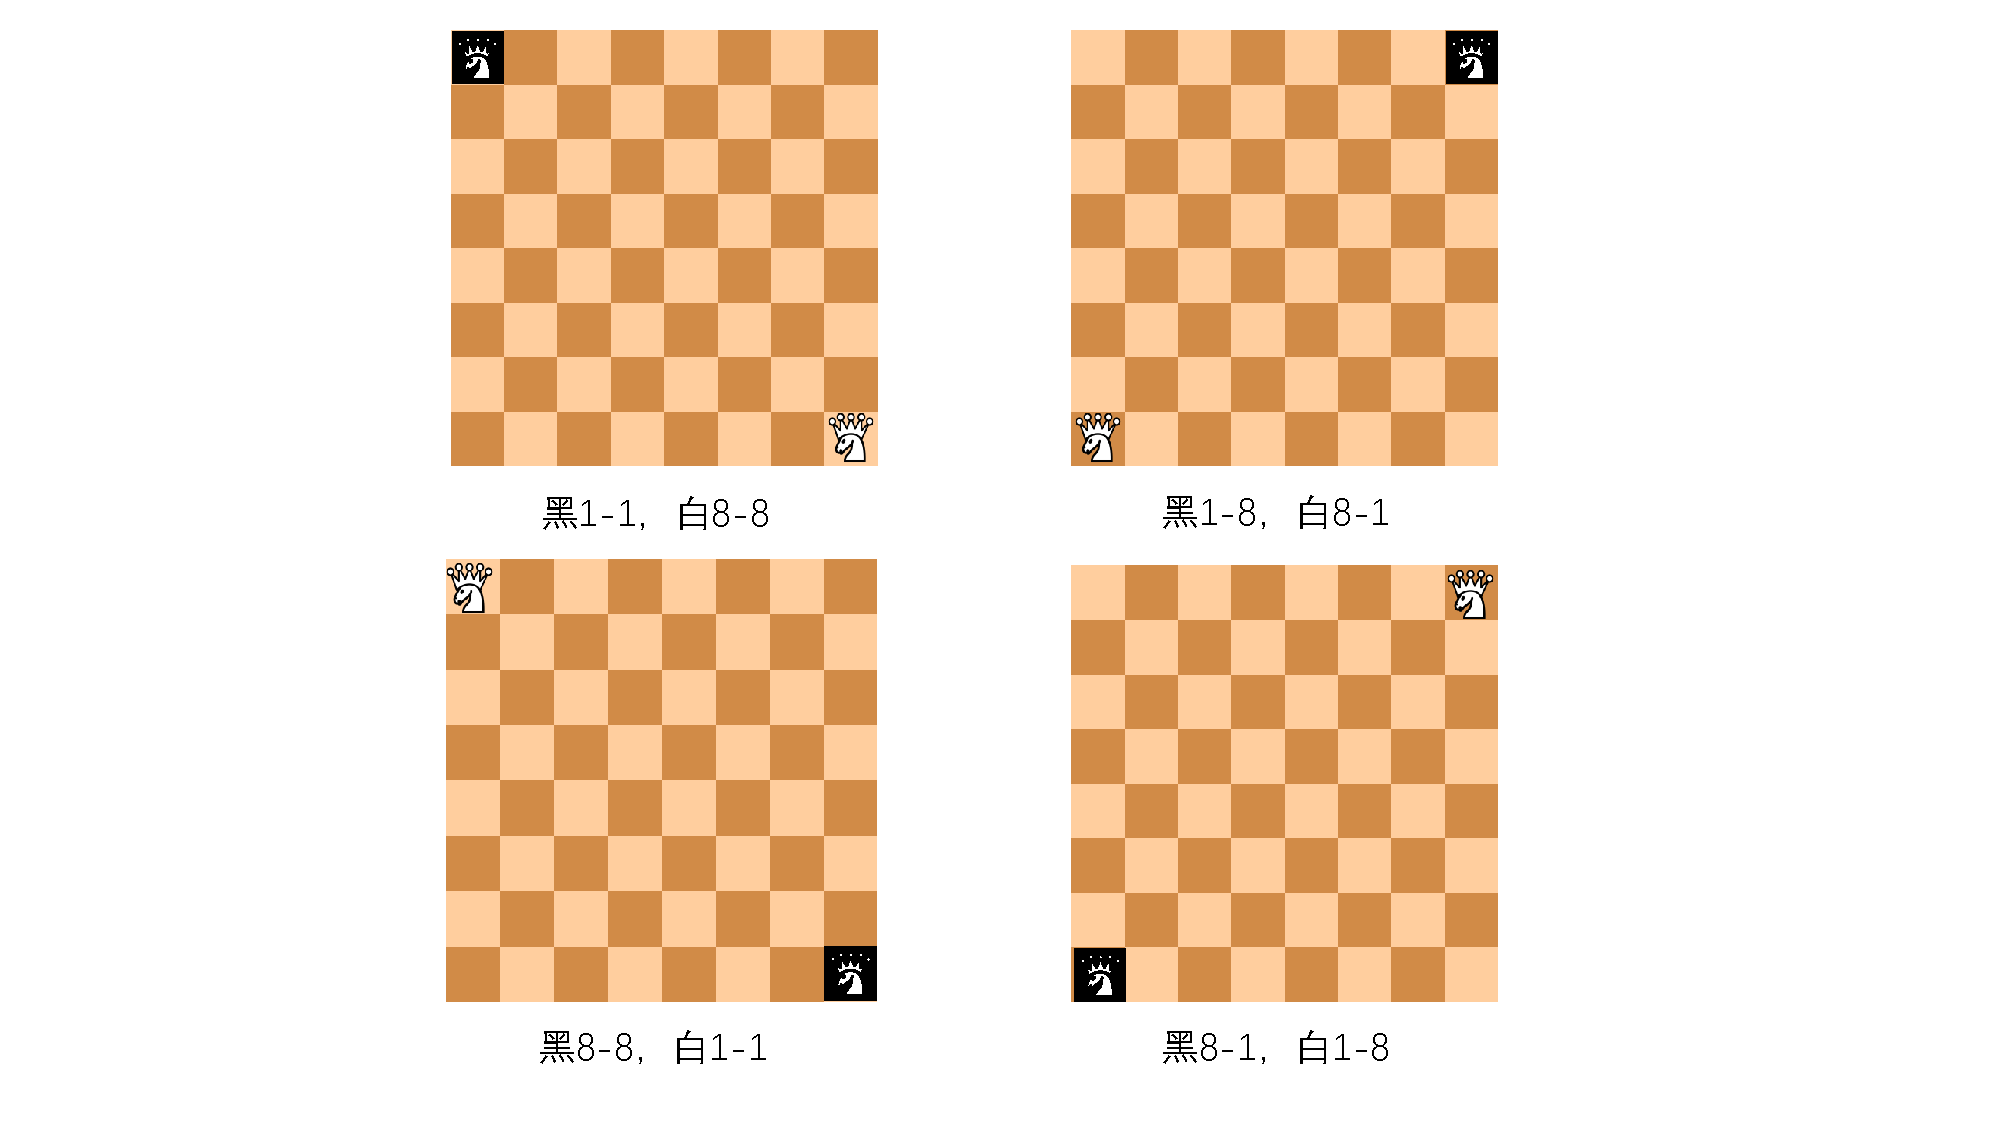
\includegraphics[width=1\textwidth]{sstate.pdf}
    \caption[sstate]{%
        超级皇后对战的4种开局%
      }
    \label{fig:sstate}
\end{figure}
对于随机玩家,贪婪玩家与~alpha-beta~剪枝玩家这三个基准玩家而言,在任意规则下,其强度排序为
\begin{equation*}
    \text{alpha-beta剪枝玩家} > \text{贪婪玩家} > \text{随机玩家} ,
\end{equation*}
具体对局胜率如表~\ref{table:baseresult}~所示,不同开局的对战结果合并统计,先手与后手分开统计,包含骑士、皇后与超级皇后三种规则状态,随机玩家简写作RP,贪婪玩家简写作GP,~alpha-beta~剪枝玩家简写作ABP。
% \begin{figure}[htb]
%     \centering
%     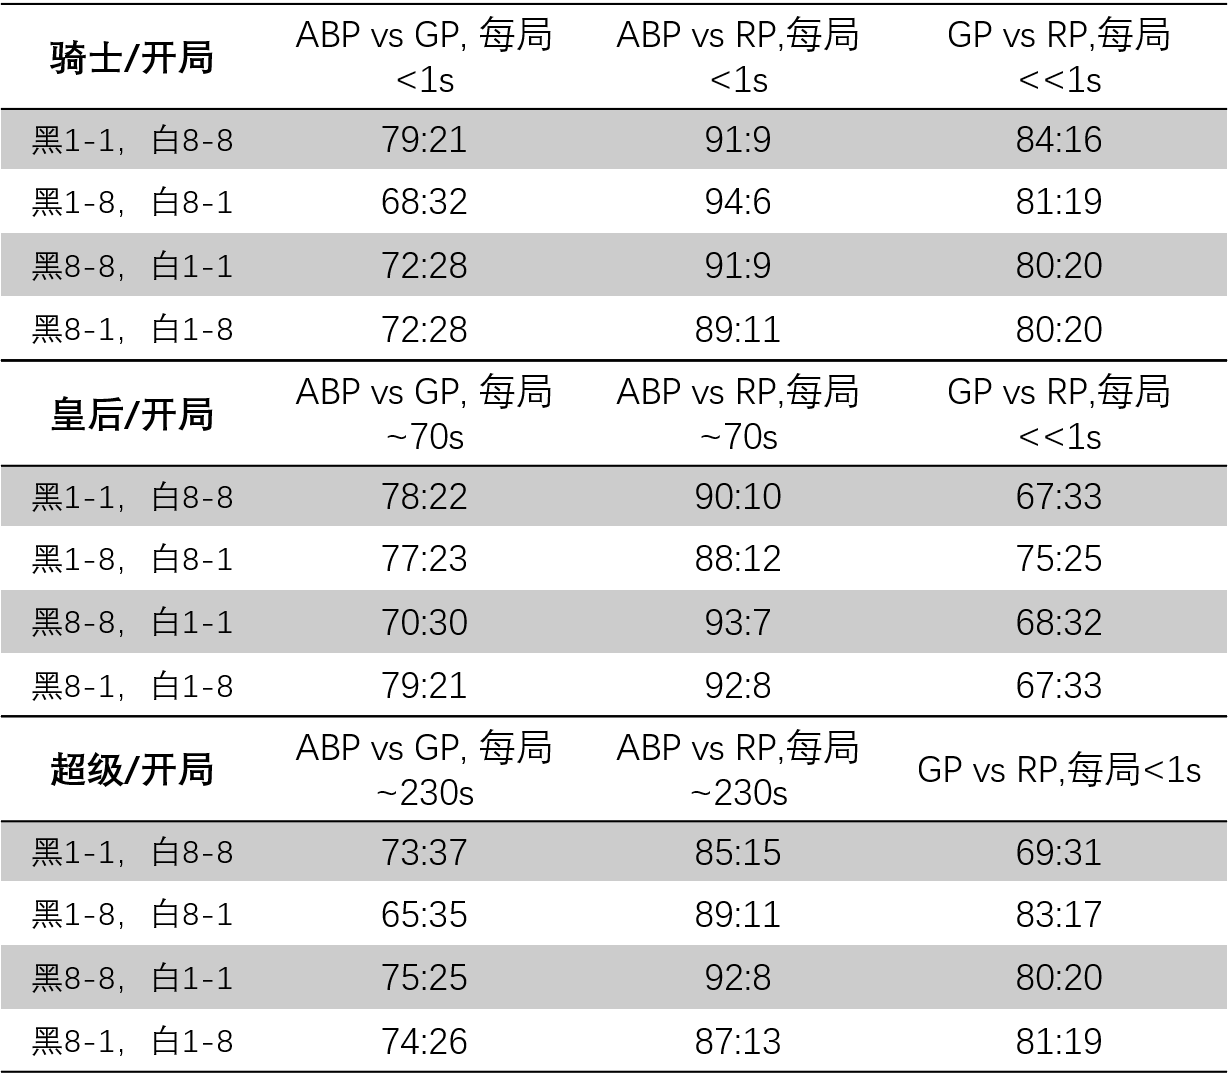
\includegraphics[width=0.8\textwidth]{baseplayer.PNG}
%     \caption[baseresult]{%
%         基准玩家测试%
%       }
%     \label{fig:baseresult}
% \end{figure}
\begin{table}[htb]
    \centering
    \caption[baseresult]{基准玩家胜率数据}
    \begin{tabular}{p{2cm}<{\centering} p{4cm}<{\centering} p{4cm}<{\centering} p{4cm}<{\centering}}
    \hline
    骑士/开局 & ABP vs GP, 每局用时~<1s & ABP vs RP,每局用时~<1s & GP vs RP,每局用时~<<1s \\ \hline
    先手 & $77\%$ & $97\%$ & $81\%$\\ 
    后手 & $64\%$ & $87\%$ & $75\%$\\ \hline
    皇后/开局 & ABP vs GP, 每局用时$\approx$70s & ABP vs RP,每局用时$\approx$70s & GP vs RP,每局用时~<1s \\ \hline
    先手 & $79\%$ & $93\%$ & $72\%$\\ 
    后手 & $78\%$ & $85\%$ & $70\%$\\ \hline
    超级/开局 & ABP vs GP, 每局用时$\approx$230s & ABP vs RP,每局用时$\approx$230s & GP vs RP,每局用时~<1s \\ \hline
    先手 & $78\%$ & $94\%$ & $73\%$\\ 
    后手 & $73\%$ & $86\%$ & $71\%$\\ \hline
    \end{tabular}
    \label{table:baseresult}
  \end{table}
从基准玩家测试结果中,我们发现贪婪玩家与~alpha-beta~剪枝玩家不能完全碾压随机玩家,随机玩家总能赢少部分局。可能的原因是在有限时间内~alpha-beta~剪枝层数不够深,陷入了局部最优解,封死了自己在后续的优势。当然也可能是因为在游戏中后期棋盘状态复杂度降低,随机玩家可以走出关键棋从而制胜。并且先手玩家会取得一定优势,先手胜率大于后手胜率。
整体上来看,~alpha-beta~剪枝玩家对随机玩家胜率在$90\%$,对贪婪玩家胜率在$75\%$,贪婪玩家对随机玩家胜率在$74\%$。
\section{强化学习训练}
我们分别训练了骑士,皇后,超级皇后三种规则下的基于经典卷积模型并使用MCTS的强化学习AI。考虑到棋盘复杂度与设备算力限制,我们仅训练超级皇后的基于深度残差网络并使用MCTS的强化学习AI。
在训练过程中,我们设置超参数如下:
\paragraph{棋局对弈生成次数}
在每一轮新的迭代中,在自我对弈过程中使用前一轮训练出的网络指导蒙特卡洛树进行对弈生成更为稳健的对弈棋盘数据并对整个棋面局势数据集进行汰旧换新。我们将其设置为40,也就是说其将进行40次自我对弈,每次对弈开局为图\ref{fig:sstate}的任意一种开局;
\paragraph{MCTS模拟步数}
使用神经网络输出的概率分布与获胜预测值指导进行MCTS过程中的搜索模拟次数,即其完成选择-扩展-反向传播的次数。我们将其设置为50。
\paragraph{置信上界常数}
在选择动作(selection)中的常数$c$,用以平衡高胜率与低访问次数的关系,决定探索力度。我们将其设置为1。
\paragraph{对战次数}
更新后的神经网络与更新前的神经网络各自指导MCTS进行若干局对弈,若更新后的神经网络胜率超过$60\%$,则其将在下一轮训练中使用新的神经网络进行自我对弈并继续指导MCTS,继续增强走棋能力。否则继续使用更新前的神经网络。我们将其设置为40。
\paragraph{神经网络超参数}
优化器学习率(learning rate)设置为0.001,丢弃率(dropout)设置为0.3,epoch数设置为20,批次容量(batch\_size)设置为128。


在数据生成时,为了使模型泛化能力更强,即在对称开局或先后手不同时表现一致,我们会对棋盘数据进行数据增强操作:对棋盘进行旋转与镜像,如图~\ref{fig:datar}。数据会因此被扩充8倍,大大增强数据集的鲁棒性。
\begin{figure}[H]
    \centering
    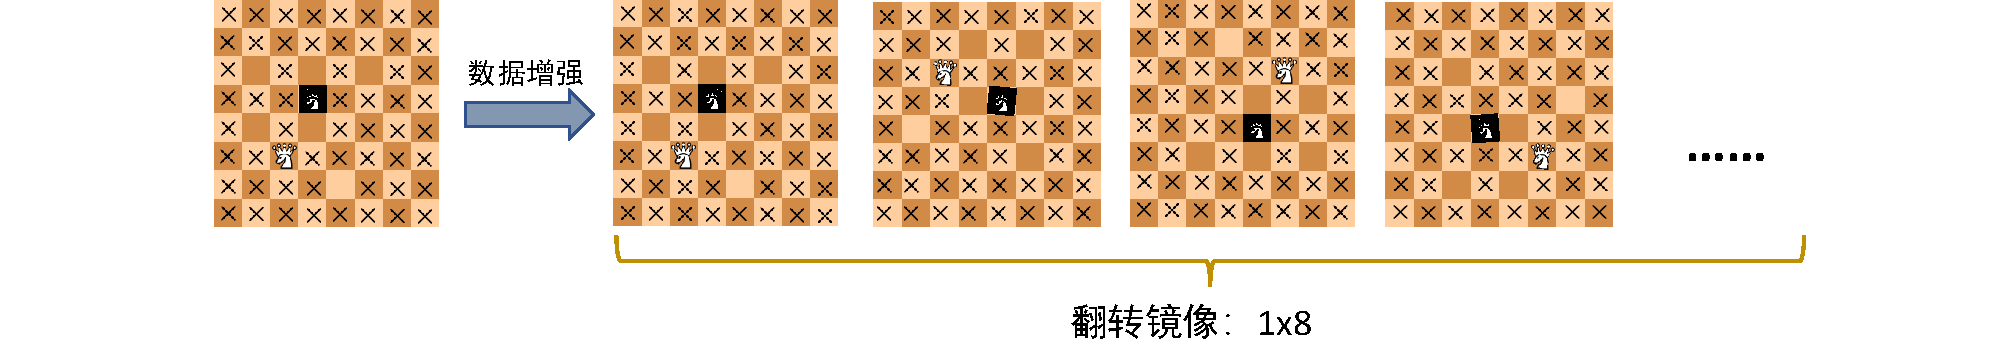
\includegraphics[width=1\textwidth]{datar.pdf}
    \caption[datar]{%
        数据增强%
      }
    \label{fig:datar}
\end{figure}
对于经典卷积模型,训练参数相对较少,训练时间花费相对较少,在使用~2080Ti~单卡进行训练时,在皇后与超级皇后规则下100轮强化学习迭代花费时间为4-5天,在骑士规则下100轮强化学习迭代花费时间为3天左右;
而对于深度残差网络而言,其网络深度与训练参数量较大,所花费时间较多,在超级皇后规则下100轮强化学习花费时间为8天左右。在实验中我们发现,在训练过程中MCTS模拟步数设置越大,则训练结果也更好,所需要的训练时间也越长。

\section{强度测试}

\subsection{经典卷积神经网络}
在现有的迭代次数下选择最好的模型结果,分别为迭代225次的超级皇后模式AI,迭代191次的皇后模式AI与迭代139次的骑士模式AI,让其与基准玩家们进行对弈测试。基于经典卷积神经网络的强化学习玩家(简写为RLP1)胜率结果如表~\ref{table:airesult}~所示。
\begin{table}[H]
    \centering
    \caption[airesult]{强化学习玩家胜率数据}
    \begin{tabular}{p{2cm}<{\centering} p{4cm}<{\centering} p{4cm}<{\centering} p{4cm}<{\centering}}
    \hline
    骑士/开局 & RLP1 vs ABP, 每局用时$\approx$50s & RLP1 vs GP,每局用时$\approx$30s & RLP1 vs RP,每局用时$\approx$30s \\ \hline
    先手 & $83\%$ & $98\%$ & $99\%$\\ 
    后手 & $71\%$ & $85\%$ & $87\%$\\ \hline
    皇后/开局 & RLP1 vs ABP, 每局用时$\approx$160s & RLP1 vs GP,每局用时$\approx$110s & RLP1 vs RP,每局用时$\approx$110s \\ \hline
    先手 & $64\%$ & $87\%$ & $94\%$\\ 
    后手 & $63\%$ & $85\%$ & $88\%$\\ \hline
    超级/开局 & RLP1 vs ABP, 每局用时$\approx$310s & RLP1 vs GP,每局用时$\approx$120s & RLP1 vs RP,每局用时$\approx$120s \\ \hline
    先手 & $59\%$ & $78\%$ & $89\%$\\ 
    后手 & $53\%$ & $74\%$ & $86\%$\\ \hline
    \end{tabular}
    \label{table:airesult}
  \end{table}
可以看到,虽然经典卷积神经网络下的各规则模型都优于基准玩家,但由于游戏的规则对先手方有优势(可用空间总是相对较多),基准玩家的走棋对于胜负存在较大的随机性影响,因此几乎没有出现强化学习玩家碾压基准玩家的情况。
在骑士与皇后规则下,强化学习玩家大幅超越基准玩家。但在超级皇后规则下,在迭代次数较多的情况下强化学习玩家强度仅仅轻微超过~alpha-beta~剪枝玩家,训练效果较差。
\subsection{深度残差网络}
我们仅使用深度残差网络训练超级皇后模式下的强化学习玩家。在现有的迭代次数下选择最好的模型结果为迭代40次的AI,让其与基准玩家们进行对弈测试。强化学习玩家(简写为RLP2)胜率结果如表~\ref{table:airesult2}~所示。
\begin{table}[H]
    \centering
    \caption[airesult2]{强化学习玩家胜率数据}
    \begin{tabular}{p{2cm}<{\centering} p{3cm}<{\centering} p{3cm}<{\centering} p{3cm}<{\centering} p{3cm}<{\centering}}
    \hline
    超级/开局 & RLP2 vs RLP1, 每局用时$\approx$250s & RLP2 vs ABP, 每局用时$\approx$350s & RLP2 vs GP,每局用时$\approx$170s & RLP2 vs RP,每局用时$\approx$170s \\ \hline
    先手 & $67\%$ & $81\%$ & $87\%$ & $98\%$\\ 
    后手 & $64\%$ & $78\%$ & $83\%$ & $95\%$\\ \hline
    \end{tabular}
    \label{table:airesult2}
  \end{table}

深度残差网络在超级皇后规则下取得了较好的结果,说明其学到了更为复杂的超级皇后对战棋局特征,相比于经典卷积神经网络效果更为理想。

